\section{Durchführung und Auswertung}

\subsection{Charakterisierung des Pumplasers}



\subsubsection{Aufbau und Durchführung}

\subsubsection{Auswertung}

\begin{figure}[H]
\begin{center}
  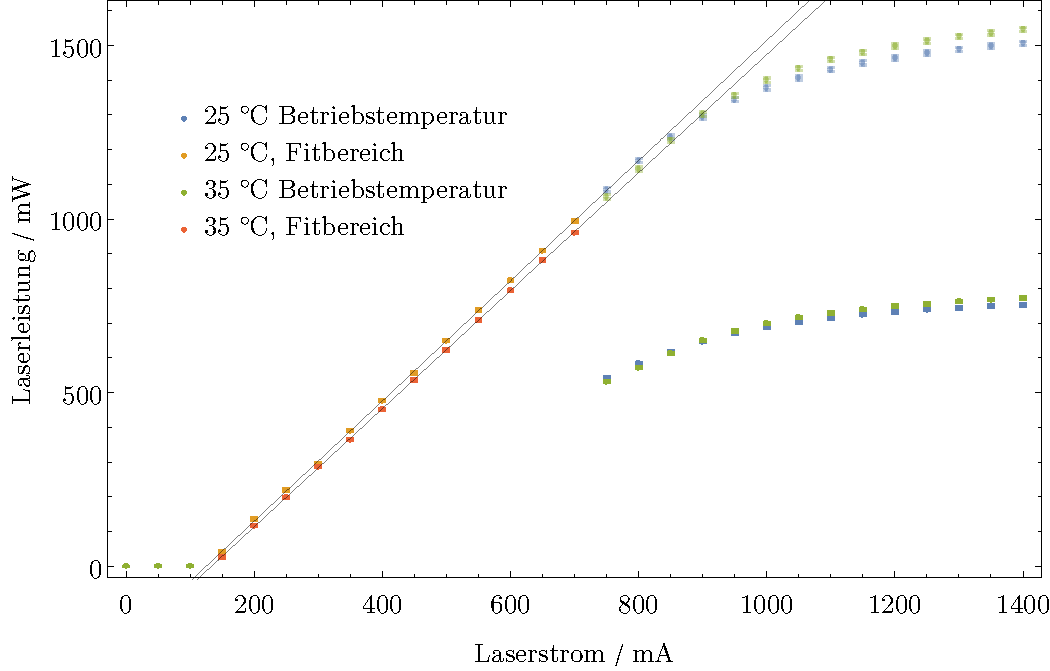
\includegraphics[width=\textwidth]{../img/PI_blau.pdf}
  \caption{PI-Kennlinie des blauen Pumplasers bei 25\grad und 35\grad
  Betriebstemperatur. Der modulationsfreie Bereich wurde linear gefittet, um
  Laserschwelle und Effizienz zu bestimmen. Im Bereich der Modulation mit einer
  Pulsweite von 50\,\% über 700\,mA Laserstrom ist durch eine
  Multiplikation mit Faktor 2 angedeutet, bei welcher Leistung der Laser
  transient betrieben wird.}
  \label{img:PI_blau}
\end{center}

\end{figure}

 